\documentclass[12pt]{article}
\usepackage[left = 0.6in, right = 0.6in, top = 0.6in, bottom = 1.5in]{geometry} 
\usepackage{enumerate, pgfplots, fontawesome5, booktabs, xcolor, hyperref, amsmath,amsthm,amssymb,amsfonts, fancyhdr, color, comment, graphicx, environ, actuarialsymbol}
\pagestyle{fancy}
\setlength{\headheight}{65pt}
%%%%%%%%%%%%%%%%%%%%%%%%%%%%%%%%%%%%%%%%%%%%%
\lhead{}
\rhead{Differentiation and functions 1}
%%%%%%%%%%%%%%%%%%%%%%%%%%%%%%%%%%%%%%%%%%%%%
%%%%%%%%%%%%%%%%%%%%%%%%%%%%%%%%%%%%%%%%%%%%%
\newcommand{\emptygrid}[3]{ % #1: range, #2: y-label, #3: "labels" or "nolabels"
    \begin{tikzpicture}
    \begin{axis}[
        axis lines = middle,
        xlabel = $x$,
        ylabel = $#2$,
        xmin=-#1, xmax=#1,
        ymin=-#1, ymax=#1,
        grid = both,
        grid style = {line width=.1pt, draw=gray!30},
        xtick distance = 5,
        ytick distance = 5,
        minor tick num = 4,
        tick label style = {font=\tiny},
        width=8cm, height=8cm,
        axis equal image,
        % Logic to hide labels if #3 is "nolabels"
        xticklabels={ \ifx\empty#3\empty\else\ifnum\pdfstrcmp{#3}{nolabels}=0 \else \fi\fi },
        yticklabels={ \ifx\empty#3\empty\else\ifnum\pdfstrcmp{#3}{nolabels}=0 \else \fi\fi }
    ]
    \end{axis}
    \end{tikzpicture}
}
%%%%%%%%%

\begin{document}
\section{Quick revision of differentiation }
Differentiate the following: (The first question of exam 1 is almost \textbf{always} differentiation)
\begin{itemize}
    \item $x^{3} + 2x - 1$
    \item $3x^{2}\sin(2x)$
    \item $e^{x}\cos(x)$
    \item $3\tan(x)$ (Do this using quotient rule)
    \item $\ln(x^{2} + 1)$
\end{itemize}

\section{Functions}
\begin{itemize}
    \item whats a mapping/relation? A fixed map of inputs to outputs from an input set to an output set (draw a quick diagram)
    \vspace{3cm}

    \item Whats a function? A mapping from one set to another that is one-to-\_\_\_ (many/one)
    \item How do we write a function? $f: Dom \to \mathbb{R}: f(x) = \dots$
    \begin{itemize}
        \item $\mathbb{R}$ here is NOT the range!! DO NOT mistake it for the range. (It is a bigger set that the range lives in, called a \textit{codomain})
    \end{itemize}
    \item Whats a Domain and Range?
    \begin{itemize}
        \item Domain: Set of all \textbf{possible} inputs
        \item Range: Set of all \textbf{actual} outputs
        \item eg: $f: \mathbb{R} \to \mathbb{R}: f(x) = x^{2}$
    \end{itemize}
    \item Whats an implied domain? When you are given a function without a domain specified, the implied domain is the \textbf{largest} possible domain that makes the function work.
    \begin{itemize}
        \item eg: $f(x) = \frac{1}{x}$
        \item eg: $g(x) = \sqrt{x-3}$
    \end{itemize}
\end{itemize}





\newpage

Some more definitions:
\begin{itemize}
    \item one to one vs one to many functions:
    \vspace{3cm}
    
    \item odd and even functions
    \vspace{3cm}

    \item Continuity: A function that is continuous has no breaks, jumps or holes in it.
\end{itemize}




\begin{align*}
f: (-\infty, a] \to \mathbb{R}, f(x) = x^{3}+2x^{2} 
\end{align*}
For what values of $a$ is $f$ a one to one function?

\vspace{3cm}






\newpage

\subsection{Hybrid/piecewise functions}
A function with different expressions over different parts of the domain
eg:
\begin{enumerate}
    \item 
\begin{align*}
f(x) = \begin{cases}
x^{2}, & x < 0 \\
2x + 1, & x \geq 0
\end{cases}
\end{align*}

Think of this as a function made up of two parts. 
\begin{enumerate}[(a)]
    \item Plot $f$
    
    \emptygrid{3}{f}{labels}
    \item Is $f$ continuous everywhere?
\end{enumerate}
\vspace{3cm}
\item 
\begin{align*}
g(x) = \begin{cases}
x^{2} & x < a\\
e^{x} & \text{elsewhere}
\end{cases}
\end{align*}

\begin{enumerate}[(a)]
    \item Are there any values of $a$ that makes $g$ continuous everywhere? 
\end{enumerate}


\end{enumerate}



\section{Addition of ordinates review}

adding $y$-values for a given $x$-value

    Consider graphing $f: (0 , 2\pi ) \to \mathbb{R}, f(x) = \frac{x^{2}}{10} + \sin(x)$

    \begin{center}
    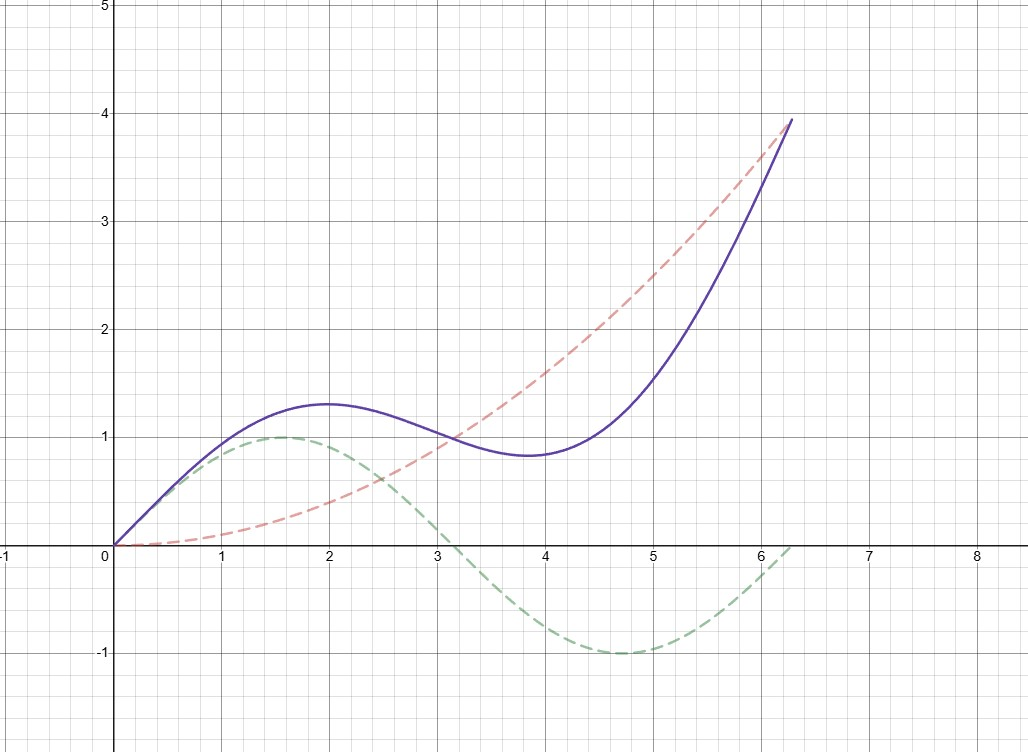
\includegraphics[scale = 0.5]{img1.jpg}
    \end{center}

strategy?
\begin{itemize}
    \item start with finding key points of each curve (if there are any)
    \item plot the curves individually
    \item add the height of each curve at discrete intervals (i.e at every tick )
    \item make sure the y values at key points match
\end{itemize}

New way to think of dilation from the y axis! i.e : $f(x) = 2x^{2} = x^{2} + x^{2}$


\newpage

Sketch the following, and then double check with your calculator
\begin{itemize}
    \item $p(x) = 2x + \sqrt{x}$
    \item $q(x) = e^{-x} + 3x $
    \item  $f: (-2\pi , 2\pi ) \to \mathbb{R}, f(x) = \sin(x) + \cos(2x)$
\end{itemize}

\begin{center}
\emptygrid{10}{p}{labels}
\emptygrid{10}{q}{labels}
\emptygrid{10}{f}{labels}
\end{center}


\newpage 

\section{Composite functions}

A function inside another function/

A function passed into another function/

A function inputted into another function/

A function of a function


Let $f(x)  = x^{2} + 2x$, and $g(x) = (x-1)^{2}$
\begin{itemize}
    \item Before: $f(x)  = x^{2} + 2x$
    \begin{itemize}
        \item $x$ was inputted into $f$ and evaluated according to the rule $x^{2} + 2x$
        \item eg: to get $f(2)$: $f(2) = 2^{2} + 2(2) = 4 + 4 = 8 $
    \end{itemize}
    \item $f(g(x))$ means
    
\begin{align*}
x \longrightarrow g(.) \longrightarrow f(.)
\end{align*}
eg: To find $f(g(2))$
\begin{align*}
2 & \longrightarrow g(2) = (2-1)^{2} = 1 \\
  & \longrightarrow f(1) = 1^{2} + 2(1) = 3\\
\text{i.e } & f(g(2)) = f(1) = 3
\end{align*}

To simplify $f(g(x))$, we substitute $g(x)$ into $f$ wherever we see an $x$:
\begin{align*} 
f(g(x)) & = f((x-1)^{2}) \\
         & = ((x-1)^{2})^{2} + 2((x-1)^{2}) \\
         & = (x-1)^{4} + 2(x-1)^{2}
\end{align*}

Try to simplify $g(f(x))$.
\end{itemize}
\newpage

\subsection{When composite functions can exist}

Consider $f: \mathbb{R} \to \mathbb{R}, f(x) = 2x-4$ and $g: \mathbb{R} \to \mathbb{R}, g(x) = \sqrt{x}$
\begin{itemize}
    \item Simplify $f(g(x))$.
    \item Simplify $g(f(x))$.
    \item Find $f(g(1))$
    \item Find $g(f(1))$
\end{itemize}

Sometimes the output values from the inner function cannot be taken by the outer function. In those cases the composite function does not exist.

Then when does $g(f(x))$ exist?
\begin{itemize}
    \item When $Ran f \subseteq Dom g$
    \item i.e The values that $f$ outputs must be within the domain of $g$
\end{itemize}

\begin{enumerate}
    \item $f(x) = \sqrt{x - 2}$, $g(x) = 3x + 12$ Does $f \circ g$ exist over $\mathbb{R}$?
    \begin{itemize}
        \item $f \circ g$ ('f of g') is another way to write $f(g(x))$
    \end{itemize}
    \vspace{4cm}


    \item We can restrict the domain of $g$ so that $f \circ g$ exists. Find a suitable domain.
    \vspace{4cm}
    
    \item $f(x) = \ln{x}$, $g(x) = x^{2} - 4$ 
    \begin{enumerate}
        \item Find a suitable domain for $g$ s.t $f \circ g$ exists.
        \item Find a suitable domain for $f$ s.t $g \circ f$ exists.
    \end{enumerate}

\end{enumerate}
\newpage



\end{document}